% =============================================================================
% Title Page – titolo in alto, sottotitolo, pannello scuro con filo oro
% =============================================================================
\begin{titlepage}
	\thispagestyle{empty}
	
	% Sfondo a tutta pagina
	\AddToShipoutPictureBG*{%
		\AtPageLowerLeft{\makebox[\paperwidth][c]{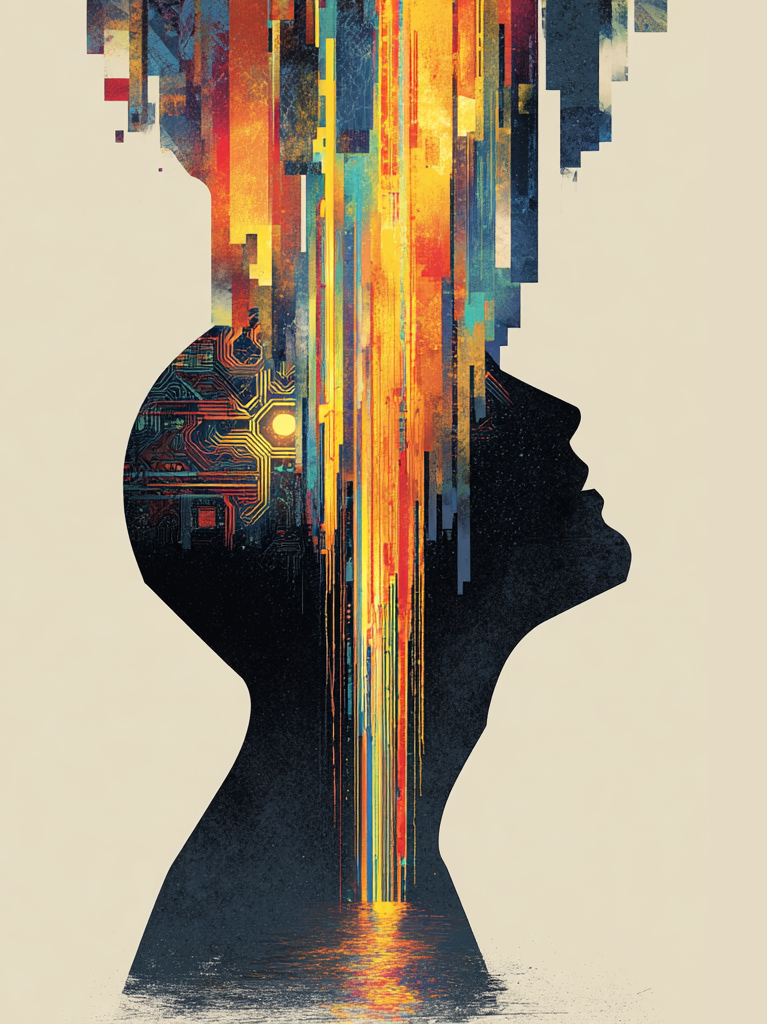
\includegraphics[height=\paperheight,keepaspectratio=false]{Cover.png}}}%
	}
	
	% --- BLOCCO TITOLO + SOTTOTITOLO SU PANNELLO SCURO ---
	% Pannello quasi opaco (blu notte) con filo oro: testo bianco/oro ben leggibile
	% anche sulla parte piu' colorata dell'illustrazione.
	\begin{tikzpicture}[remember picture,overlay]
		\node[
		anchor=north,
		align=center,
		yshift=-1.6cm,          % distanza dal bordo superiore
		text=white,
		fill=covernight,
		fill opacity=.86,       % pannello scuro, appena trasparente
		text opacity=1,
		draw=covergold,
		draw opacity=1,
		line width=1.1pt,
		rounded corners=6pt,
		inner xsep=20pt,
		inner ysep=18pt,
		text width=.80\paperwidth
		] at (current page.north) {%
			% Titolo (= \booktitle, a capo forzato): Playfair Display bianco, grande
			{\coverdisplayfont\fontsize{40}{44}\selectfont\bfseries\spaceskip=0.26em plus 0.1em minus 0.08em\relax\color{white}Memorie di un\\futuro anteriore\par}
			\vspace{0.9em}
			{\color{covergold}\rule{0.35\linewidth}{1.2pt}\par}
			\vspace{0.9em}
			% Sottotitolo: serif corsivo, bianco, piu' grande
			{\fontsize{13.5}{18}\selectfont\itshape\color{white}
				\subtitleA\\[0.5em]\subtitleB\par
			}
			\vspace{1.1em}
			{\color{covergold}\large\sffamily\bfseries\textls[160]{\MakeUppercase{\authorname}}\par}
		};
		
		% --- CHIP EDITORE: leggermente più in basso ---
		%\node[
		%anchor=south,
		%fill=black,
		%text=white,
		%rounded corners=6pt,
		%inner xsep=10pt,
		%inner ysep=6pt
		%] at ([yshift=6mm]current page.south) {\large\sffamily\textls[50]{\MakeUppercase{\publisher}}};
	
	\end{tikzpicture}
	
\end{titlepage}
